% run the command ' lualatex -shell-escape Reference.tex ' twice in the terminal to visualize table of contents
\documentclass[twoside]{article}
\usepackage[utf8]{inputenc}
\usepackage[english]{babel}
\usepackage{geometry}
\usepackage{multicol}
\usepackage{minted}
\usepackage{python}
\usepackage[hidelinks]{hyperref}
\usepackage{fancyhdr}
\usepackage{listings}
\usepackage{pdfpages}
\usepackage{needspace}
\usepackage{sectsty}
\usepackage{array}
\usepackage{multirow}
\usepackage{longtable}
\usepackage{xcolor}
\usepackage{afterpage}
\usepackage{amssymb}
\usepackage{amsmath}
\usepackage[inline]{enumitem}

\geometry{letterpaper, portrait, left=0.5cm, right=0.5cm, top=1.8cm, bottom=1cm}

\sectionfont{\Huge\bfseries\sffamily}

\setminted{
    style=tango,
    breaklines=true
}

\setlength{\headsep}{0.5cm}
\setlength{\columnsep}{0.5cm}
\setlength{\columnseprule}{0.01cm}
\renewcommand{\columnseprulecolor}{\color{gray}}

\pagestyle{fancy}
\pagenumbering{arabic}
\fancyhead{}
\fancyfoot{}
\fancyhead[LO,RE]{\textsf{First, solve the problem. Then, write the code.}}
\fancyhead[LE,RO]{\textsf{\leftmark}}
\fancyfoot[LE,RO]{\textbf{\textsf{\thepage}}}

\renewcommand{\headrulewidth}{0.01cm}
\renewcommand{\footrulewidth}{0.01cm}

\setlength{\parindent}{0em}
% column space
\setlength{\tabcolsep}{10pt} % Default value: 6pt
% upper and lower padding
\renewcommand{\arraystretch}{1.5} % Default value: 1

\definecolor{prussianblue}{rgb}{0.0, 0.19, 0.33}
\definecolor{indigo(dye)}{rgb}{0.0, 0.25, 0.42}
\definecolor{lapislazuli}{rgb}{0.15, 0.38, 0.61}
\definecolor{mediumelectricblue}{rgb}{0.01, 0.31, 0.59}
\definecolor{smalt(darkpowderblue)}{rgb}{0.0, 0.2, 0.6}
\definecolor{yaleblue}{rgb}{0.06, 0.3, 0.57}
\definecolor{skobeloff}{rgb}{0.0, 0.48, 0.45}
\definecolor{pinegreen}{rgb}{0.0, 0.47, 0.44}

\begin{document}
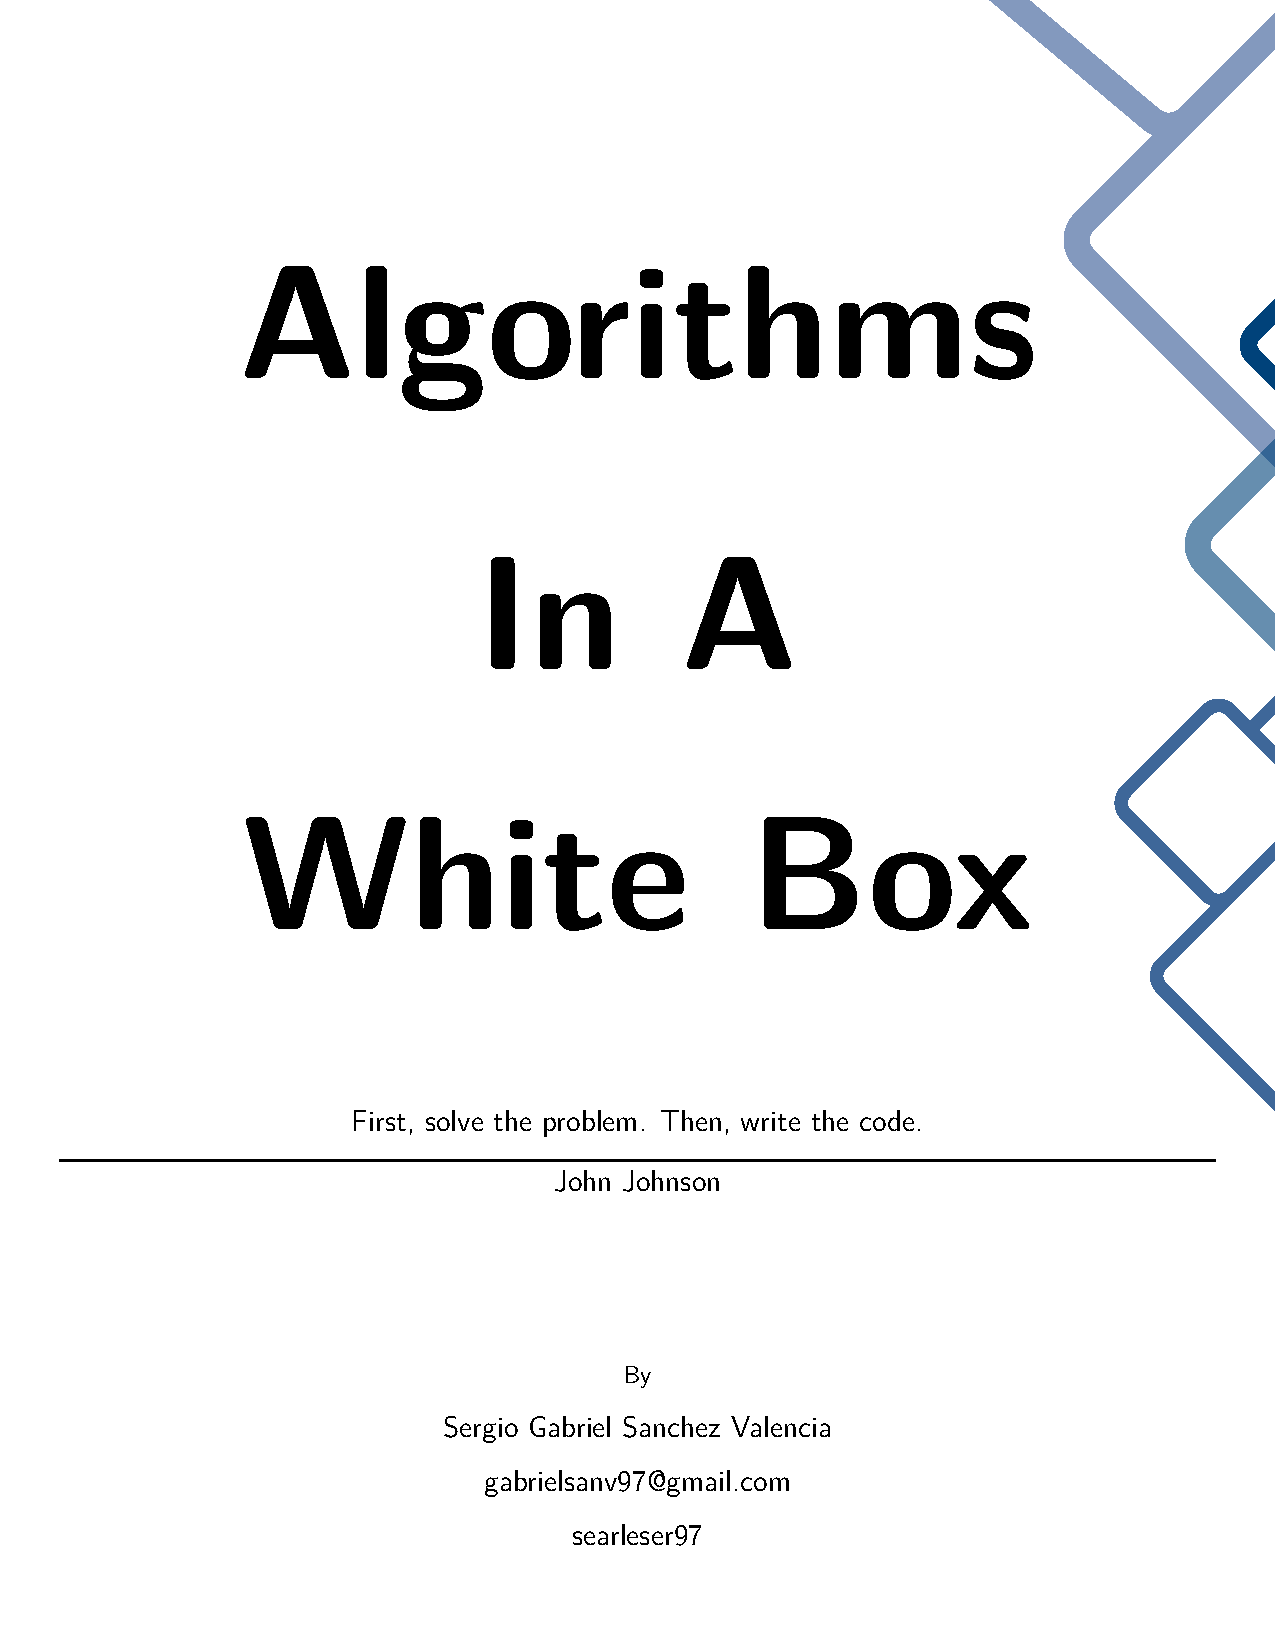
\includepdf{"/home/san/Projects/Algorithms-In-A-White-Box/LaTex Template/TitlePage/TitlePage.pdf"}
\null
\thispagestyle{empty}
\newpage
\fontfamily{lmss}
\selectfont
\begin{multicols*}{2}
	\tableofcontents
	\newpage
	\cleardoublepage
	\end{multicols*}
\sectionfont{\bfseries\sffamily\centering\Huge}
\vspace{1em}
\section*{BITs Manipulation}
\markboth{BITS MANIPULATION}{}
\addcontentsline{toc}{section}{BITs Manipulation}
\vspace{3em}
\subsectionfont{\large\bfseries\sffamily\underline}
\subsection*{Least Significant Set Bit}
\addcontentsline{toc}{subsection}{Least Significant Set Bit}
First thing we need to notice is that when we add 1 to a number $N$, what we are doing is just converting the first (right to left) 0-bit into a 1-bit and the 1-bits before get converted to 0-bits because $1 + 1 = 0$ with carry of $1$ in binary, therefore we will be having a carry of 1-bit until we find a 0-bit.\\

\textbf{Example:}

$$00100111 + 1 = 00101000$$

Second thing we need to notice is very simple, lets start by denoting $\overline{N}$ as $N$ with all it's bits inverted (1-bits change to 0-bit and viceversa), if we perform an $AND$ operation between $N$ and $\overline{N}$ we will get all bits in $0$ as result.\\

\textbf{Example:}

$$N = 00100111$$
$$\overline{N} = 11011000$$

So, to achieve our main objective which is to extract the least significant bit (rightmost bit) we can just invert $N$ and add 1 to it that will convert the first 0-bit to 1-bit so if we make an $AND$ operation with $N$ and $\overline{N}$ we get everything before the lsb as 0-bit and after the lsb we also get everything as 0-bit.\\

And we can write this as the 2's complement since what we did was just to invert bits and add one, which is just the exact definition of 2's complement.\\

\textbf{C++ Code:}\\

\begin{minted}[bgcolor=LightGray]{cpp}
int lsb(int n) {
  return n & -n;
}
\end{minted}
\begin{multicols*}{2}
\end{multicols*}
\sectionfont{\bfseries\sffamily\centering\Huge}
\vspace{1em}
\section*{Ranges}
\markboth{RANGES}{}
\addcontentsline{toc}{section}{Ranges}
\vspace{3em}
\subsectionfont{\bfseries\sffamily\centering\LARGE}
\vspace{0em}
\subsection*{Data Structures}
\addcontentsline{toc}{subsection}{Data Structures}
\vspace{2em}
\subsubsectionfont{\large\bfseries\sffamily\underline}
\subsubsection*{BIT}
\addcontentsline{toc}{subsubsection}{BIT}
\subsection{What is a Binary Indexed Tree}

Binary Indexed Tree (BIT) or Fenwick Tree is a data structure that can efficiently update
elements and compute prefix sums in an array.\\

It supports query and update in $O(lg(N))$ time with $O(N)$ space complexity and it requires just a few lines of code!

\subsection{Idea}



\begin{multicols*}{2}

\end{multicols*}
\end{document}
